\chapter{Single Input Multiple Output Line of Sight Channel}

this system uses a multiple antennas at the \Rx to decrease the probability of error in the communication system, and that's a type of Spatial Diversity.

\section{\Rx antenna array}
in a SIMO communication system, we send the message from a \Tx with one antenna and receive it with multiable antennas \Rx.

the structure (the way the antennas are arranged) called the antenna array.
by using the two built-in functions 'phased.ULA' and 'getElementPosition', we can make a liner antenna array and get the coordinates for each antenna.

\subsection{Scatteringchanmtx}
as we did in SISO LOS, we will repeat it for each system because we need scattering channel matrix to calculate the BER.
the difference here is we will replace the single antenna we put as the \Rx with the antenna array we made in the previous step.

\section{Bit Error Rate (BER)}
we will calculate it this time for the SIMO system.

to monitor the relationship between Eb/No and BER in a SIMO LOS channel so will use the 11 values of Eb/No and calculate the BER for each one using helpMIMOBER function.
\vfill

\begin{figure}[!h]
	\centering
	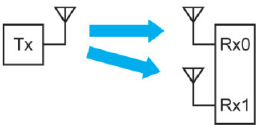
\includegraphics[width=0.4\linewidth]{figures/SIMO}
	\caption{SIMO}
\end{figure}

\newpage
\section{Plotting}
to see the difference between SISO and SIMO we will plot the both of them on the same graph.

as we can see in Figure[\ref{SISO and SIMO BER for each Eb/No}], the BER decreases as we increase the Eb/No for each SISO and SIMO.

but the SIMO curve is steeper than the SISO one, which indicates a better BER for SIMO over SISO.

\begin{figure}[!h]
	\centering
	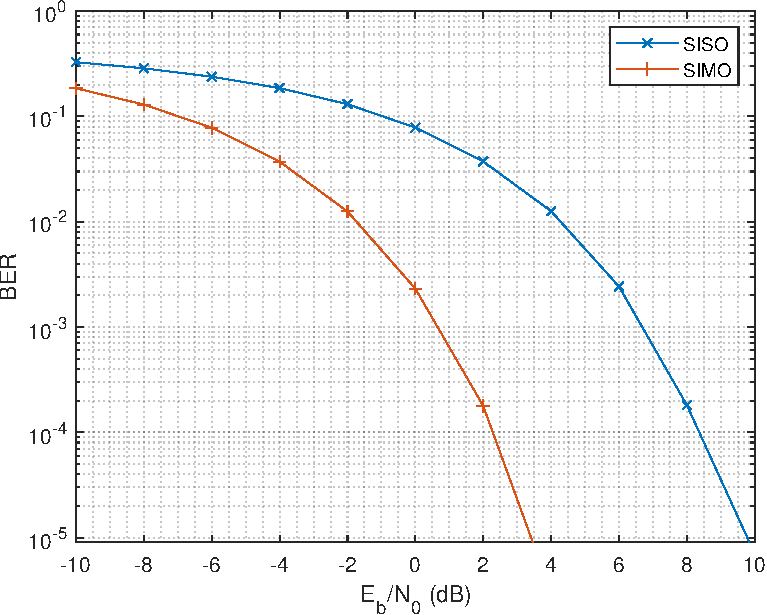
\includegraphics[width=1\linewidth]{figures/SISO_SIMO_BER}
	\caption{}
	\label{SISO and SIMO BER for each Eb/No}
\end{figure}


\newgeometry{margin=0pt}
\newpage
\vfill
\begin{figure}
	\centering
	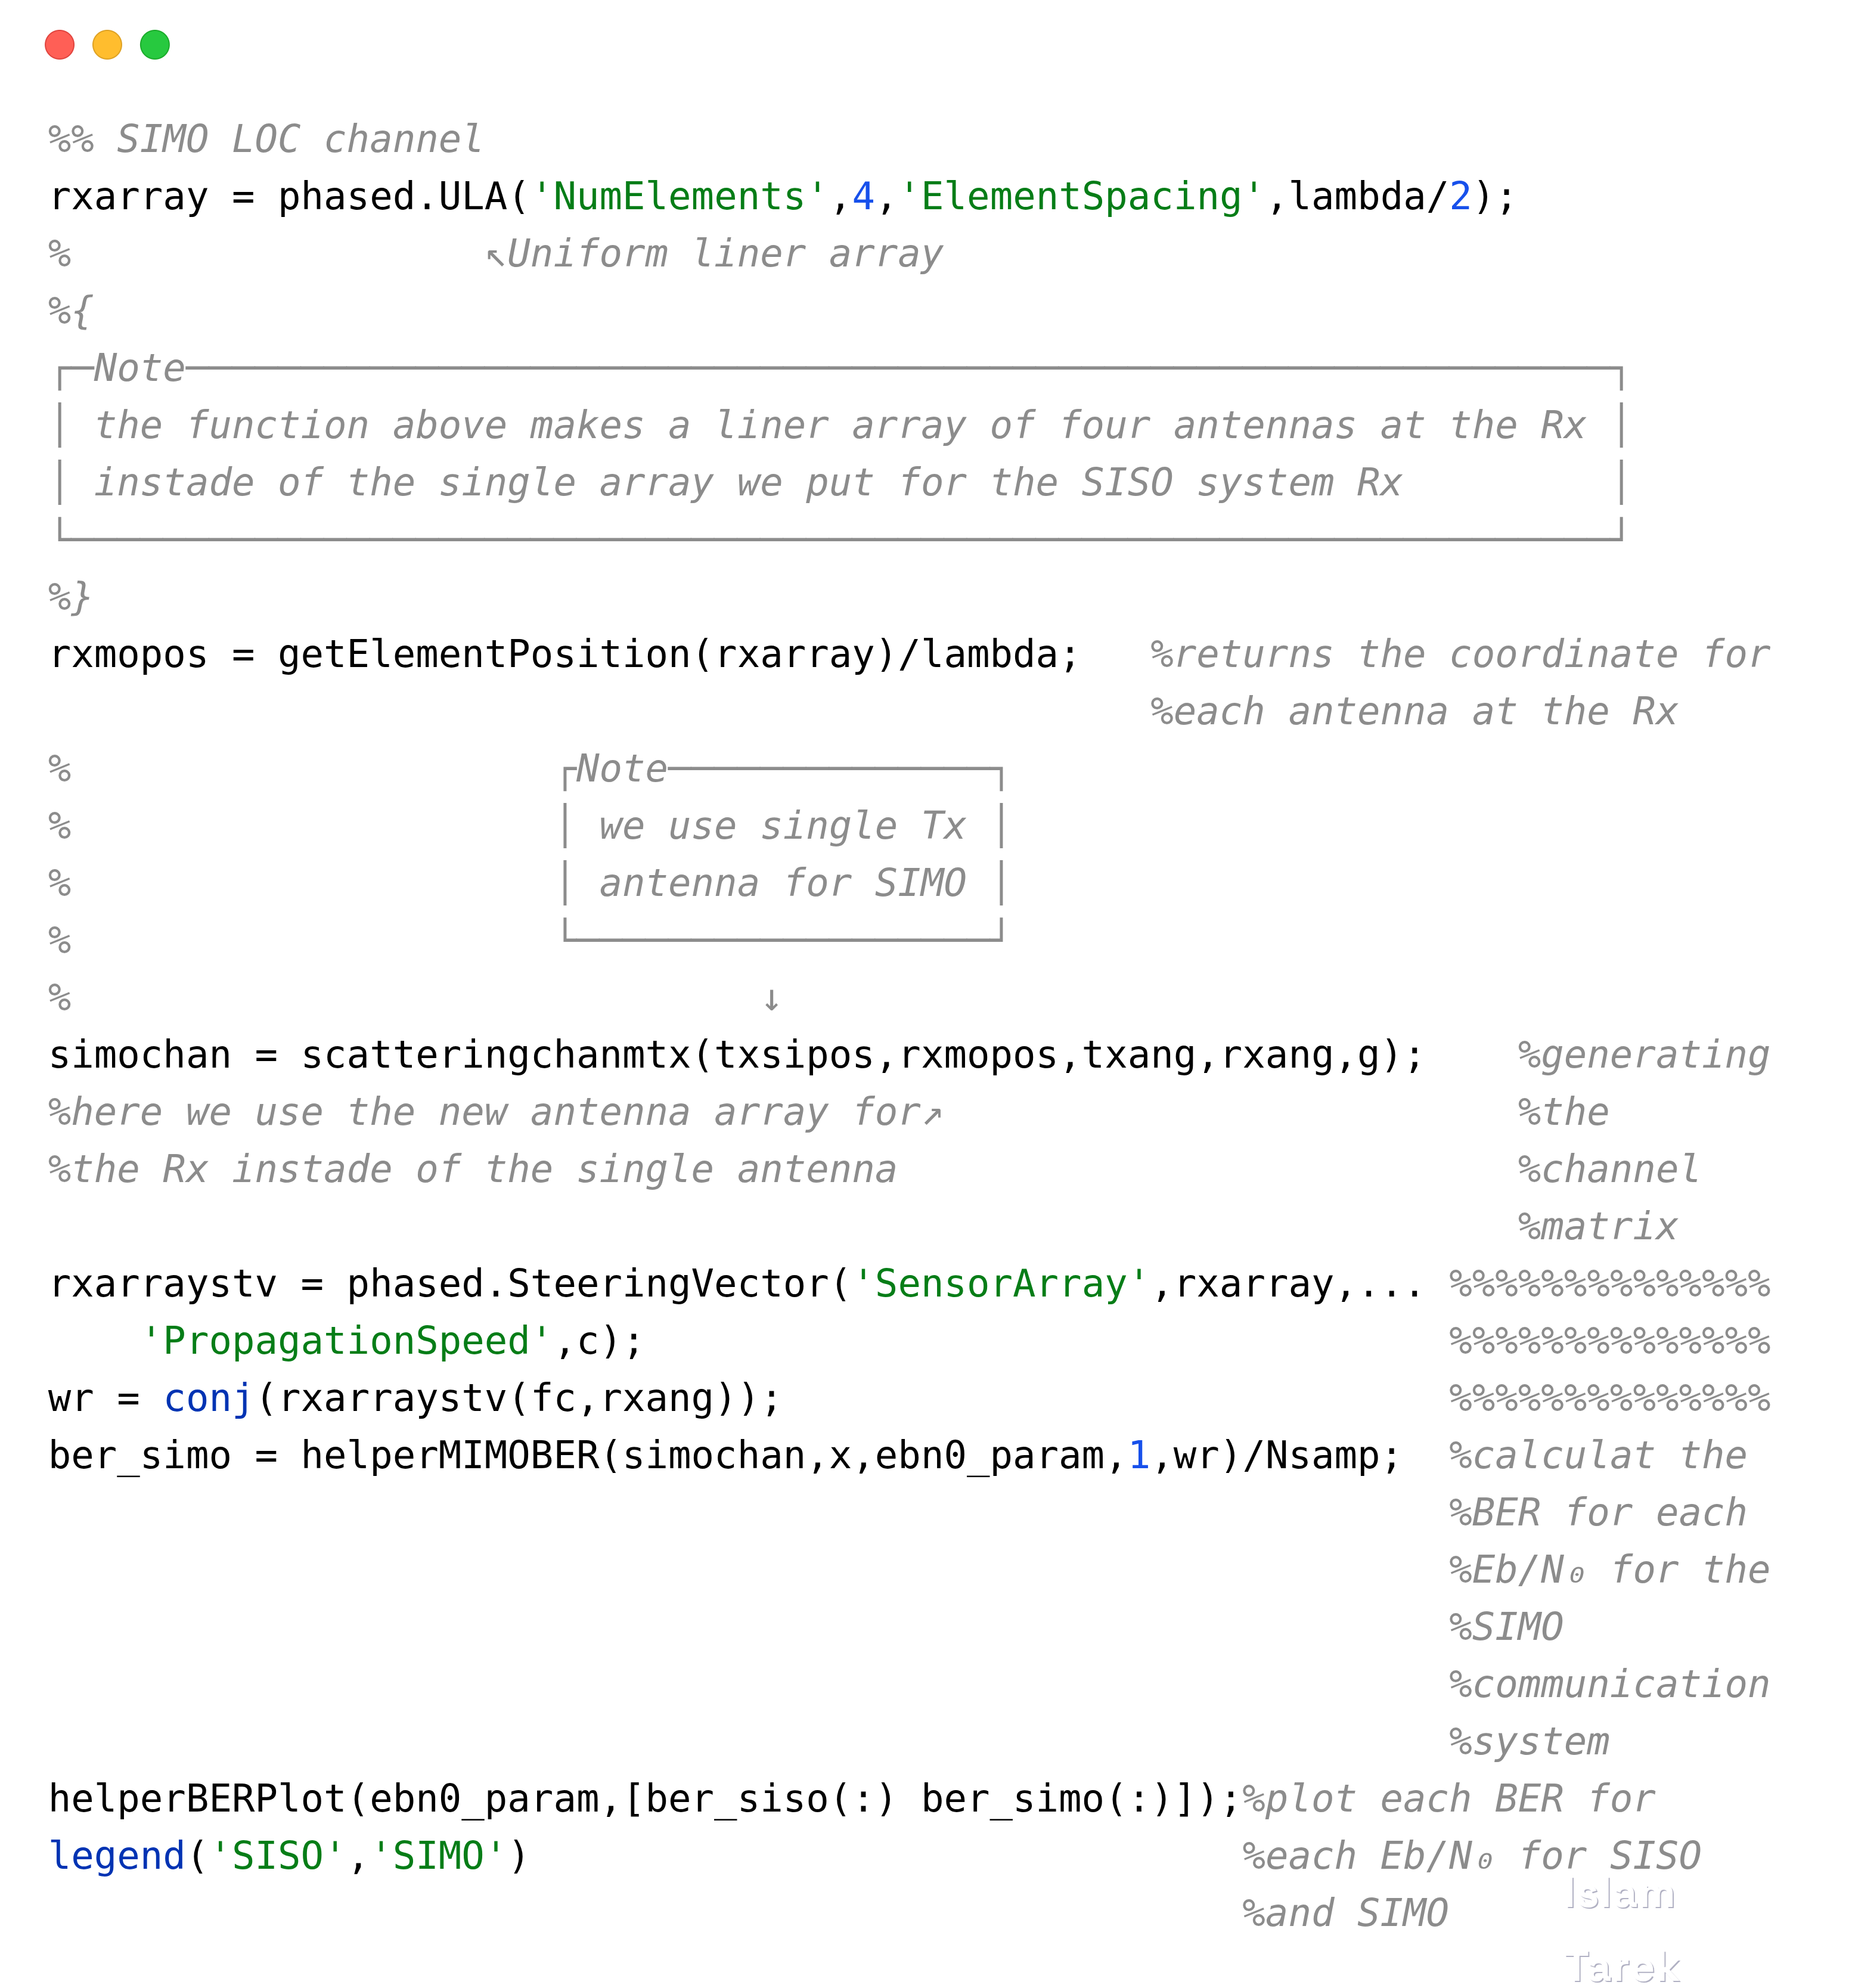
\includegraphics[width=0.7\linewidth]{figures/code3}
\end{figure}
\vfill
\restoregeometry